\documentclass[german,10pt]{book}      
\usepackage{makeidx}
\usepackage{babel}            % Sprachunterstuetzung
\usepackage{amsmath}          % AMS "Grundpaket"
\usepackage{amssymb,amsfonts,amsthm,amscd} 
\usepackage{mathrsfs}
\usepackage{rotating}
\usepackage{sidecap}
\usepackage{graphicx}
\usepackage{color}
\usepackage{fancybox}
\usepackage{tikz}
\usetikzlibrary{arrows,snakes,backgrounds}
\usepackage{hyperref}
\hypersetup{colorlinks=true,
                    linkcolor=blue,
                    filecolor=magenta,
                    urlcolor=cyan,
                    pdftitle={Overleaf Example},
                    pdfpagemode=FullScreen,}
%\newcommand{\hyperref}[1]{\ref{#1}}
%
\definecolor{Gray}{gray}{0.80}
\DeclareMathSymbol{,}{\mathord}{letters}{"3B}
%
\newcounter{num}
\renewcommand{\thenum}{\arabic{num}}
\newenvironment{anmerkungen}
   {\begin{list}{(\thenum)}{%
   \usecounter{num}%
   \leftmargin0pt
   \itemindent5pt
   \topsep0pt
   \labelwidth0pt}%
   }{\end{list}}
%
\renewcommand{\arraystretch}{1.15}                % in Formeln und Tabellen   
\renewcommand{\baselinestretch}{1.15}                 % 1.15 facher
                                                      % Zeilenabst.
\newcommand{\Anmerkung}[1]{{\begin{footnotesize}#1 \end{footnotesize}}\\[0.2cm]}
\newcommand{\comment}[1]{}
\setlength{\parindent}{0em}           % Nicht einruecken am Anfang der Zeile 

\setlength{\textwidth}{15.4cm}
\setlength{\textheight}{23.0cm}
\setlength{\oddsidemargin}{1.0mm} 
\setlength{\evensidemargin}{-6.5mm}
\setlength{\topmargin}{-10mm} 
\setlength{\headheight}{0mm}
\newcommand{\identity}{{\bf 1}}
%
\newcommand{\vs}{\vspace{0.3cm}}
\newcommand{\noi}{\noindent}
\newcommand{\leer}{}

\newcommand{\engl}[1]{[\textit{#1}]}
\parindent 1.2cm
\sloppy

         \begin{document}  \setcounter{chapter}{0}


\chapter{Physik des Klimas I\\Solarkonstante und Paleoklima}
% Kap x
\label{chap_Klima1}

Unser Klima wird in erster Linie durch die Sonne bestimmt. Von ihr stammt die Energie,
die nahezu s\"amtliche dynamischen Vorg\"ange auf der Erde antreibt. 
Eine zweite Energiequelle besteht in Zerfallsprozessen radioaktiver Elemente im Erdinneren.
Diese Energieform k\"onnen wir jedoch f\"ur das Verst\"andnis des Klimas vernachl\"assigen.

Die Energieform, die in der Sonne durch Kernfusionsprozesse entsteht - streng genommen sollte
man nat\"urlich immer von \glqq Umwandlung\grqq\ sprechen, d.h., bei Kernfusionspozessen wird
Kernenergie in thermische (Bewegungs-)Energie, Strahlungsenergie sowie in Neutrinos umgewandelt -, 
erreicht uns in Form 
von elektromagnetischer Strahlung, haupts\"achlich im sichtbaren Bereich. Die Oberfl\"ache der
Sonne hat eine Temperatur von rund 5800\,Kelvin und die zugeh\"orige thermische Strahlung
hat ihr Maximum bei rund 500\,nm, das entspricht Licht im gr\"un-blauen Bereich. 

Der erste Abschnitt wird auf die Solarkonstante eingehen, d.h., die Menge an Energie, die pro
Zeiteinheit (Sekunde) und pro Fl\"acheneinheit (Quadratmeter) bei der Erde oberhalb der
Atmosph\"are ankommt. In diesem Zusammenhang gehen wir auch auf Ph\"anomene wie die Albedo
der Erde ein. Au\ss erdem betrachten wir verschiedene Faktoren, die in der Vergangenheit
einen Einfluss auf die Solarkonstante bzw.\ die Einstrahlung der Sonnenstrahlung auf die
Erde gehabt haben und damit unser Klima beeinflusst haben k\"onnten.
Schlie\ss lich betrachten wir auch kurz das Gebiet der Pal\"aoklimatologie, das sich mit
dem Klima im Verlauf der Geschichte der Erde besch\"aftigt. 


\section{Die Solarkonstante}

Die Solarkonstante ist definiert als das langj\"ahrige Mittel der Intensit\"at pro Fl\"acheneinheit der 
Sonneneinstrahlung oberhalb der Erdatmosph\"are. 
Die Intensit\"at ist dabei die Energie, die pro Sekunde 
auf eine bestimme Fl\"ache - in diesem Fall ein Quadratmeter senkrecht zur Strahlungsrichtung - trifft
(siehe Abb.\ \ref{fig_solar_constant}). 
Die IAU (International Astronomical Union) hat 2015 die Solarkonstante aufgrund neuerer
Messungen auf den Wert
\begin{equation}
               S = 1361\,{\rm J \cdot s^{-1} \cdot m^{-2}}
\end{equation}
festgelegt. In \"alteren B\"uchern findet man oft den Wert $S= 1367\,{\rm J \cdot s^{-1} \cdot m^{-2}}$, der
von 1982 bis 2015 G\"ultigkeit hatte. Heute misst man die Solarkonstante mit Satelliten, wobei die
gemessenen Intensit\"aten auf den mittleren Abstand Erde-Sonne - die Astronomische Einheit - 
umgerechnet wird.

\begin{SCfigure}[30][htb]
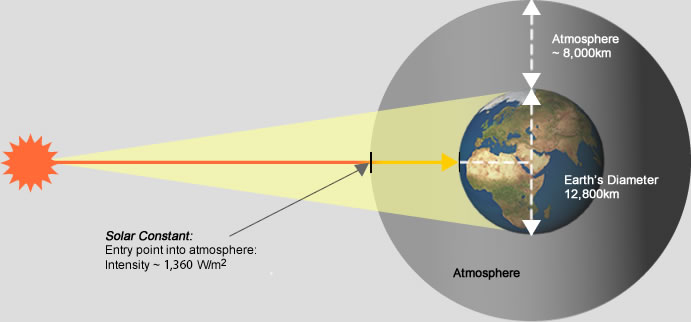
\includegraphics[scale=0.4]{./Bilder/solar-constant.jpg}
\caption{\label{fig_solar_constant}%
Definition der Solarkonstanten. Die gemessene Intensit\"at der Sonnenstrahlung
oberhalb der Erdatmosph\"are wird auf den mittleren Abstand Sonne-Erde umgerechnet.
(aus \cite{Solar})}
\end{SCfigure}


\subsection{Sonnenaktivit\"at}

Streng genommen handelt es sich bei der Solarkonstanten nicht um eine Naturkonstante. Sie unterliegt
kleinen Schwankungen. Eine winzige Schwankung entsteht durch den 11-Jahres-Zyklus der 
Sonnenaktivit\"at. Im sichtbaren Bereich machen diese Schwankungen aber nur rund 0,1\% aus. Lediglich
im UV- bzw.\ im R\"ontgen-Bereich k\"onnen diese Schwankungen wesentlich gr\"o\ss er sein, allerdings
wird diese Strahlung in h\"oheren Schichten unserer Atmosph\"are reflektiert bzw.\ absorbiert und 
erreicht den Erdboden gr\"o\ss tenteils nicht. Allerdings lassen sich Schwankungen in
der mittleren Jahrestemperatur von der Gr\"o\ss enordnung von $0,1^\circ$C mit einer Periode von 11
Jahren \"uber l\"angere Zeitr\"aume nachweisen. 
Au\ss erdem gab es in der Vergangenheit h\"aufiger Perioden, in denen die Sonne
insgesamt weniger aktiv war und die m\"oglicherweise zu kleinen Eiszeiten gef\"uhrt haben. Bekannt sind solche
Perioden in der Zeit zwischen dem 14.\ und 18.\ Jahrhundert (das sogenannte Sp\"orer-Minimum und das
Maunder-Minimum; wobei ein direkter Bezug zum Klima in dieser Periode immer noch umstritten ist), 
beispielsweise durch Wintergem\"alde von 
Pieter Bruegel dem \"Alteren und seinen S\"ohnen. 

Seit Beginn des 17.\ Jahrhunderts (seit der Erfindung des
Teleskops) wurden die Sonnenflecken direkt beobachtet, sodass es gute Aufzeichnungen
gibt. F\"ur die Perioden davor eignen sich manche Isotopmessungen (z.B.\ ${}^{14}$C und ${}^{10}$Be).
Diese Isotope entstethen haupts\"achlich in der Atmosph\"are durch den Einfluss der kosmischen Strahlung, 
die wiederum durch eine starke Sonnenaktivit\"at und die damit verbundenen Sonnenwinde 
abgeschw\"acht wird. Dies f\"uhrt zu einer Korrelation zwischen der H\"aufigkeit dieser Isotope in
Bohrproben, die auf bestimmte Zeiten datiert werden k\"onnen, und der Sonnenaktivit\"at: H\"ohere
Isotopenanteile lassen auf geringere Sonnenaktivit\"at schlie\ss en, da zu diesen Zeiten die kosmische
Strahlung ungehinderter in die Atmosph\"are dringen konnte.

\subsection{Milankovi\'c-Zyklen}

F\"ur unser Klima (vermutlich)
relevante Schwankungen sind die sogenannten Milankovi\'c-Zyklen, benannt nach
dem serbische Mathematiker Milutin Milankovi\'c (1879-1958). Hierbei handelt es sich um regelm\"a\ss ige
Oszillationen in den Parametern der Erdumlaufbahn um die Sonne. Bei diesen Parametern handelt
es sich insbesondere um die Exzentrizit\"at der Erdbahn, die Neigung der Erdachse und die
Pr\"azession der Erdachse.

\subsubsection{Die Exzentrizit\"at der Erdumlaufbahn} 

In einem reinen Zwei-K\"orper-Problem mit einer $1/r^2$-Kraft
(manchmal als nicht-relativistisches Kepler-Problem bezeichnet) bewegt sich ein leichter K\"orper (Erde)
um einen schweren K\"orper (Sonne) auf einer elliptischen Bahn, wobei sich der schwere K\"orper
in einem der Brennpunkte der Ellipse befindet. Dies gilt ganz allgemein f\"ur die Relativkoordinate
zwischen den beiden Himmelsk\"orpern, auch wenn die Masse des leichteren Himmelsk\"orpers
im Vergleich zu dem schwereren Himmelsk\"orper nicht vernachl\"assigt werden kann.  

Durch den Einfluss der anderen Planeten, insbesondere Jupiter und Saturn, ver\"andert sich die 
Bahnkurve der Erde jedoch im Verlauf der Zeit. Insbesondere kann auch die Exzentrizit\"at der
elliptischen Bahn zwischen einer fast kreisf\"ormigen Erdumlaufbahn ($\epsilon = 0,0006$) und einer
schwach elliptischen Bahn ($\epsilon =0,058 $) variieren \cite{Wikipedia_Milankovic}. 
Diese Werte schwanken periodisch mit einer Periode von rund
405\,000 Jahren, wobei auch Unterzyklen von der Gr\"o\ss enordnung von 100\,000 Jahren existieren. 

Derzeit betr\"agt der Wert rund $\epsilon= 0,0167$, was einer Schwankung in der Entfernung zwischen
Erde und Sonne im Bereich zwischen
147,09 Millionen Kilometern und 152,10 Millionen Kilometern entspricht. Obwohl die Differenz in diesen
Werten nur rund 3.4\% ausmacht, bedeutet dies f\"ur die Intensit\"at der Sonnenstrahlung
eine Schwankung von rund 6,8\% im Verlauf eines Jahres \hyperref[Anm-1]{(1)}. 
Bei einer entsprechend gr\"o\ss eren Exzentrizit\"at sind auch diese 
Schwankungen gr\"o\ss er und k\"onnen bis zu 24\% ausmachen.

\subsubsection{Neigung der Erdachse} 

Im Vergleich zur Ekliptik, also der Ebene der Erdumlaufbahn
um die Sonne, ist die Drehachse der Erde um rund $23,5^\circ$ geneigt. Dieser Neigungswinkel
\"andert sich aufgrund der Einfl\"usse anderer Planeten mit einer Periode von rund 41.000 Jahren
und schwankt zwischen $22,1^\circ$ und $24,5^\circ$.

Auch diese Schwankung hat zun\"achst einen jahreszeitlichen Einfluss auf unser Klima: Ist der
Neigungswinkel gr\"o\ss er, ist der Unterschied im Einfallswinkel der Sonne zwischen Sommer und
Winter entsprechend gr\"o\ss er, d.h., die jahreszeitlichen Schwankungen fallen st\"arker aus. 
Das wiederum kann einen Einfluss darauf haben, wie stark Schnee- und Eisfl\"achen im Sommer
abtauen und sich somit zur\"uckbilden. Au\ss erdem haben diese Schwankungen einen Einfluss
auf verdunstende Wassermengen in h\"oheren Breitengraden und somit auf den dortigen Niederschlag, 
was sich beispielsweise im Winter auf erh\"ohten Schneezuwachs bei Gletschern auswirken kann. 

\subsubsection{Pr\"azession der Erdachse} 

Da die Erde keine ideale Kugelform hat sondern entlang der Erdachse
etwas abgeplattet ist, also entlang des \"Aquators etwas \glqq dicker\grqq\ als entlang von L\"angengraden
(der Abstand vom Erdzentrum zum Nord- bzw.\ S\"udpol ist um rund 21 Kilometer kleiner als der 
Abstand vom Erdzentrum zum \"Aquator, wobei hier f\"ur die Erde vereinfachend die Form eines
Rotationsellipsoids angenommen wird). Der gravitative Einfluss von Sonne und Mond (in geringerem Ma\ss\
auch der von anderen Planeten, insbesondere Jupiter und Saturn) bewirkt ein Drehmoment, das 
die Erdachse aufrichten w\"urde, falls sich die Erde nicht drehte. Wegen der Drehimpulserhaltung wird
die Drehachse zur Seite gedreht und rotiert langsam um eine Senkrechte zur Erdbahn ((Bild!)).
Diese Drehung bezeichnet man als Pr\"azession. Sie hat eine Periode von rund 25\,800 Jahren.

Der Haupteffekt der Neigung der Erdachse sind die Jahreszeiten, die auf der Nord- und S\"udhalbkugel
der Erde um ein halbes Jahr relativ zueinander verschoben sind. Die Pr\"azession bewirkt, zusammen mit
den anderen Orbitalparametern, dass die Unterschiede zwischen den Jahreszeiten (insbesondere
zwischen Sommer und Winter) hinsichtlich ihrer Intensit\"at verschieden stark ausfallen k\"onnen.
Wenn beispielsweise die Elliptizit\"at der Erbahn (d.h.\ die Exzentrizit\"at) sehr gro\ss\ ist, kann
die Richtung der Erdachse relativ zu den Hauptachsen die Strahlungsunterschiede zwischen Sommer
und Winter entweder verst\"arken (wenn der Sommer mit dem Perihel zusammenf\"allt) oder
abschw\"achen (wenn Sommer mit dem Aphel zusammenf\"allt). 

Ein weiterer wesentlicher Faktor f\"ur das Klima ist, dass die Nordhalbkugel der Erde gr\"o\ss ere
Landmassen hat als die S\"udhalbkugel, die eine gr\"o\ss ere Wasserfl\"ache hat. Insofern spielt es
eine Rolle, ob die oben erw\"ahnte Verst\"arkung der Unterschiede zwischen Sommer und Winter
f\"ur die Nord- oder f\"ur die S\"udhalbkugel zutrifft.  

W\"ahrend man in der physikalischen und astrophysikalischen Literatur f\"ur die Pr\"azession der
Erde einen Wert von 25\,800 (oder aufgerundet 26\,000) Jahren findet, findet man in der
Literatur zur Klimaphysik bzw.\ zu den Milankovi\'c-Zyklen
oftmals einen Wert von 23\,000 Jahren. F\"ur die Physik (z.B.\ die
Bestimmung des Fr\"uhlingspunkts und den damit zusammenh\"angenden Jahreszeiten) ist
die Richtung der Erdachse relativ zur Sonne wichtig. F\"ur die Klimaforschung ist man eher an der
Richtung der Erdachse relativ zum Perihel bzw.\ Aphel interessiert. Wegen der Periheldrehung
der Erde, verschieben sich diese Punkte aber langsam. Der kombinierte Effekt von 
Pr\"azession und Periheldrehung f\"uhrt zu der verk\"urzten Periode von 23\,000 Jahren. 


\subsection{Das Sonnenalter}

Auf sehr langen Zeitskalen nimmt die Solarkonstante zu: In 100 Millionen Jahren um rund 1\% 
\cite{Wikipedia_Solarkonstante}. Zu Beginn der Erdgeschichte betrug die Sonnenintensit\"at nur
rund 70\% ihres heutigen Werts. Das Klima auf der Erde h\"atte somit wesentlich k\"alter sein m\"ussen
und alles Wasser auf der Erde h\"atte gefroren sein m\"ussen. Es gibt aber deutliche Hinweise
darauf, dass es insgesamt meist w\"armer auf der Erde gewesen ist. Dies bezeichnet man als
das  \textit{Faint young Sun paradox} \cite{Wikipedia_Faint}. Eine m\"ogliche L\"osung ist, dass der
Kohlendioxidgehalt der Atmosph\"are in fr\"uheren Zeiten (z.B.\ aufgrund von Vulkanismus)
wesentlich h\"oher war als heute. Diese Frage ist aber noch nicht endg\"ultig gekl\"art.

\section{Die Albedo}

Die Albedo ist ein Ma\ss\ daf\"ur, wie stark ein Gegenstand eine Strahlung reflektiert. Es ist so etwas
wie der totale elastische Wirkungsquerschnitt eines Gegenstands f\"ur elektromagnetische Strahlung. 
Allerdings handelt es sich nicht um eine Fl\"ache, sondern um ein Verh\"altnis: das Verh\"altnis
von reflektierter Intensit\"at zu eingestrahlter Intensit\"at. Man kann die Albedo als Funktion
der Wellenl\"ange bzw.\ der Frequenz betrachten (da es um die reflektierte Strahlung geht, soll die
Wellenl\"ange bzw.\ Frequenz erhalten bleiben), meist interessiert man sich aber f\"ur die
Summe \"uber das gesamte Spektrum. 

Wenn man ein Foto von der Erde betrachtet, aufgenommen von einem Satelliten oder, besser noch, 
von einer Raumsonde oder Rakete auf dem Weg zum Mond oder einem anderen Ort im Sonnensystem,   
ist alles, was man von der Erde sieht, reflektierte Strahlung (siehe Abb.\ \ref{fig_NASA_Welt}). 
Auf einem solchen Bild sieht man
sofort, welche Teile der Erde eine hohe und welche eine niedrige Albedo haben: Schnee- und Wolkenfelder
haben eine hohe Albedo, ebenso Eisfelder; Wasser und W\"alder haben eine sehr niedrige Albedo. 
Sand bzw.\ W\"uste oder Steppen haben eine mittlere Albedo. 

\begin{SCfigure}[30][htb]
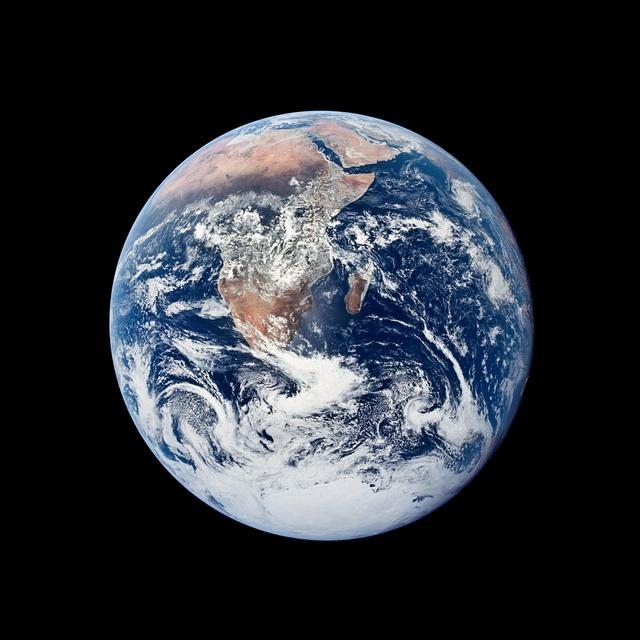
\includegraphics[trim=70 70 70 70, clip, scale = 0.3]{./Bilder/as17-Albedo_small.jpg}
\caption{\label{fig_NASA_Welt}%
Die Erde, aufgenommen von der Crew der Apollo-17 Mission im Jahre 1972. Deutlich erkennbar sind
die Antarktis, der afrikanische Kontinent, die Insel Madagaskar und die saudi-arabische Halbinsel. Die sehr
stark reflektierenden Gebiete sind wei\ss, das sind Schnee- und Wolkenfl\"achen. Die W\"usten sind
deutlich heller als Waldgebiete oder Grasfl\"achen. 
Sehr dunkel sind die Meere. Diese Helligkeiten entsprechen der
Albedo der jeweiligen Fl\"achen. (aus \cite{NASA_World})}
\end{SCfigure}

Die Albedo hat einen sehr gro\ss en Einfluss auf unser Klima. Je gr\"o\ss er die Albedo eines
Planeten ist, umso geringer ist (bei gleichbleibenden anderen Faktoren) die Oberfl\"achenerw\"armung. 
W\"ahrend die Erde insgesamt eine Albedo von 0,3 hat, hat beispielsweise der Planet Venus 
aufgrund seiner dichten Wolkenschicht eine Albedo von 0,7. Obwohl Venus deutlich n\"aher an der Sonne
ist als die Erde und aus diesem Grunde eine doppelt so hohe Solarkonstante hat, w\"are ihre
Temperatur aufgrund der Albedo k\"uhler als die der Erde. Tats\"achlich ist ihre Oberfl\"achentemperatur 
jedoch wesentlich h\"oher (bei $460^\circ$C). Der Grund ist der Treibhauseffekt: Die Atmosph\"are
von Venus besteht zu 96\% aus Kohlendioxid. 

\section{Aufbau der Atmosph\"are}

Die Atmosph\"are der Erde wird in verschiedene Schichten unterteilt, von denen die untersten
drei Schichten - die Troposph\"are, die Stratosph\"are und die Mesosph\"are - den gr\"o\ss ten
Einfluss auf unser Klima haben. Sie sind durch ihre Temperaturgradienten definiert. Die beiden
dar\"uber liegenden Schichten - die Thermosph\"are (100--600\,km) und die Exosph\"are
(600--200\,000\,km) - haben keinen direkten Einfluss auf unser Wetter bzw.\ Klima. 

\subsection{Die Troposph\"are}

Die Troposph\"are ist die unterste Atmosph\"arenschicht, in der sich nahezu alle Wettervorg\"ange
abspielen. Definiert ist sie durch einen negativen Temperaturgradienten, d.h., in dieser Schicht
nimmt die Temperatur mit der H\"ohe ab. Sie erstreckt sich an den Polen bis in eine H\"ohe von
rund 6--8\,km, in den Tropen bis zu einer H\"ohe von 12--18\,km. Im Durchschnitt hat sie eine
H\"ohe von 13\,km. 

Die Abnahme der Temperatur h\"angt mit der Druckabnahme zusammen. Der Druck nimmt
nahezu exponentiell mit der H\"ohe ab (dies gilt auch weit \"uber die Troposph\"are hinaus). Aus diesem
Grund dehnt sich aufsteigende Luft aus
(sie passt sich praktisch instantan dem Umgebungsdruck an) und wird dabei k\"uhler. Dieser
Vorgang erfolgt nahezu adiabatisch, d.h., es findet kein W\"armeaustausch mit der Umgebung
statt. Aus diesem Grund nimmt die Temperatur mit der H\"ohe ab. 

Eine instabile Wetterlage liegt
vor, wenn die Abk\"uhlung eines Luftpakets bei seinem Aufstieg aufgrund des verminderten
Drucks langsamer erfolgt, als es der Temperatur der Umgebung entspricht. In diesem Fall hat
das Luftpaket in einer bestimmten H\"ohe eine h\"ohere Temperatur als die Umgebung, aber
es hat denselben Druck. H\"ohere Temperatur aber gleicher Druck bedeutet, dass die Dichte
des Luftpakets geringer ist als die Dichte der Umgebungsluft und somit ist das Luftpaket leicher
und steigt weiter in die H\"ohe. Es findet somit eine Konvektion statt. Nimmt die Temperatur eines
Luftpakets jedoch beim Aufstieg schneller ab, als die Temperatur der Umgebung, bleibt das
Luftpaket dichter und steigt nicht weiter bzw.\ sinkt wieder. In diesem Fall ist die Lage stabil.
Insbesondere herrscht eine stabile Wetterlage bei einer Inversionslage, d.h., wenn die
Temperatur lokal mit der H\"ohe zunimmt. In aufsteigende Luft nimmt der Druck immer noch
ab, sie k\"uhlt sich somit ab und ihre Temperatur bleibt unter der Temperatur der Umgebung.
Somit ist dieses Luftpaket dichter als die Luft der Umgebung und sinkt wieder ab.   

Gehen wir an der Erdoberfl\"ache von einer mittleren Temperatur von rund $18^\circ$C aus,
so kann die Temperatur bis zur Obergrenze der Troposph\"are auf rund $-50^\circ$C bis $-60^\circ$C
abnehmen.

\subsection{Die Stratosph\"are}

Oberhalb der Troposph\"are beginnt die Stratosph\"are, wobei diese beiden Atmosph\"arenschichten
durch die sogenannte Tropopause getrennt sind. In der Stratosph\"are nimmt die Temperatur
mit zunehmender H\"ohe zu und kann in rund 50\,km H\"ohe wieder nahezu bei $0^\circ$C
liegen. In der Stratosph\"are liegt die Ozonschicht. Das Ozon absorbiert die UV-Strahlung,
was zu einer Erw\"armung f\"uhrt. Da hier die h\"oher liegenden Luftschichten eine h\"ohere
Temperatur haben, kommt es in der Stratosph\"are praktisch nicht mehr zur Konvektion. 
Wolken, z.B.\ Gewitterwolken, die bis in die Stratosph\"are reichen, bilden dort meist einen
sogenannten Amboss, d.h.\ eine flache ausgedehnte Struktur, in der keine Konvektion mehr
stattfindet. 

\subsection{Die Mesosph\"are}

Oberhalb der Stratosph\"are in rund 50--60\,km H\"ohe beginnt die Mesosph\"are. Sie reicht bis 
ungef\"ahr 80--90\,km. In dieser Schicht findet man kaum noch Ozon, sodass die Temperatur 
in der Mesosph\"are wieder abnimmt, teilweise bis deutlich unter $-140^\circ$C. Dies ist 
die k\"alteste Schicht unserer Atmosph\"are.

\subsection{Thermosph\"are und Exosph\"are}

In rund 85\,km H\"ohe beginnt die Thermosph\"are. Hier ist die Luft so d\"unn, dass
die Atome von einzelnen Photonen auf sehr hohe Geschwindigkeiten beschleunigt
werden k\"onnen, und da die mittlere Wegl\"ange der Atome bzw.\ Molek\"ule sehr
gro\ss\ ist, kommt es kaum zu einem Austausch. Die Temperatur nimmt daher wieder
zu, bis teilweise auf \"uber $1000^\circ$C. 

Oberhalb der Thermosph\"are in rund 600--700\,km H\"ohe beginnt die sogenannte
Exosph\"are. Die Temperatur \"andert sich hier nicht - die Luft wird so d\"unn, dass man
von Temperatur im thermodynamischen Sinne kaum sprechen kann. Der \"Ubergang
zwischen beiden Schichten ist flie\ss end. Eine Definition definiert die Grenze zwischen
diesen beiden Schichten \"uber die mittlere freie Wegl\"ange der Atome bzw.\ Teilchen.
Als Obergrenze der Exosph\"are wird meist die Schicht definiert, in der die Sonnenwinde
einen gr\"o\ss eren Einfluss auf die Teilchen haben als das Gravitationsfeld der Erde.
Diese Schicht liegt bei rund 200\,000\,km. 

\subsection{Homosph\"are und Heterosph\"are}

Bis zu ungef\"ahr der gleichen H\"ohe wie die Mesosp\"are, d.h.\ bis rund 85\,km, 
reicht auch die sogenannte
Homosph\"are. Das ist der Bereich der Atmosph\"are, der als \glqq well mixed\grqq\ (gut
durchmischt) gilt. In diesem Bereich \"andert sich die Zusammensetzung der Luft
kaum, d.h., in diesem Bereich besteht die Atmosph\"are 
zu rund 78\% aus Stickstoff, 21\% Sauerstoff, 0,94\% Argon   
sowie Kohlendioxid, Neon, Helium, Methan, Stickoxide und weitere Spurengase. Bis zu dieser H\"ohe
findet ausreichend vertikale Durchmischung der Luft statt, sodass diese Verh\"altnisse
bestehen bleiben. Oberhalb von rund 85\,km beginnt die Heterosph\"are. Hier ist die Luft
so d\"unn, dass es zu einer Trennung der verschiedenen Gasanteile entsprechend
ihrer molekularen Gewichte kommt. Sauerstoff, Stickstoff und Argon bleiben zun\"achst
weg, sp\"ater in gr\"o\ss erer H\"ohe auch Helium, sodass es in den \"au\ss ersten
Schichten praktisch nur noch Wasserstoff gibt. Wasserstoff und zu einem geringeren  
Anteil Helium sind auch die einzigen Gase, die dem gravitativen Einfluss der Erde
entkommen und in den Weltraum entweichen k\"onnen.



\section{Anmerkungen}

\begin{anmerkungen}
\item
\label{Anm-1}%
Der Grund f\"ur den Faktor 2 zwischen der Schwankung im Abstand und
der Schwankung in der Intensit\"at der Sonneneinstrahlung liegt in dem $1/r^2$-Gesetz
der Intensit\"at als Funktion des Abstands:
\begin{equation}
        \frac{1}{(r\pm \Delta r)^2} \approx \frac{1}{r^2} \mp 2 \frac{\Delta r}{r} \, .
\end{equation}

\end{anmerkungen}



\begin{thebibliography}{99}
\bibitem{Solar} Solarkonstante; Uni Kassel,\\
       \url{https://www.greenrhinoenergy.com/solar/radiation/images/solar-constant.jpg}         
\bibitem{NASA_World} NASA Image and Video Library, 
       \url{https://images.nasa.gov/details/as17-148-22727}
\bibitem{NASA_facts} NASA Earth Fact Sheet; 
      \url{https://nssdc.gsfc.nasa.gov/planetary/factsheet/earthfact.html}   
%\bibitem{Petty} Grant W.\ Petty; \textit{A First Course in Atmospheric Radiation}, 2nd Ed.; Sundog
%         Publishing, Madison, Wisconsin; 2006.       
\bibitem{Wikipedia_Faint} Wikipedia \glqq Faint young Sun paradox\grqq\ 
        \url{https://en.wikipedia.org/wiki/Faint_young_Sun_paradox}.                 
\bibitem{Wikipedia_Milankovic} Wikipedia \glqq Milankovitch cycles\grqq.   
       \url{https://en.wikipedia.org/wiki/Milankovitch_cycles}.        
\bibitem{Wikipedia_Solarkonstante} Wikipedia \glqq Solarkonstante\grqq.   
       \url{https://de.wikipedia.org/wiki/Solarkonstante}.               
\end{thebibliography}

\end{document}

